

\section{General Job Shop Manufacturing Systems}
\label{sec:general-job-shop}

\subsection*{Theory and Exercises}

\Opensolutionfile{hint}
\Opensolutionfile{ans}

Perhaps the term `class' needs some clarification. A network with a
single class of jobs means that all jobs have the same service
distribution at the same station. (Of course, the service rates at
different stations can be different.) In multi-class networks jobs of
different classes typically have different service distributions even
if served at the same station. Note that we do not discuss multi-class
queueing networks in this course.

There is typo in Section Zijm.2.4.3, just above Eq.2.34. There the visit ratio is defined as $V_i=\lambda_{i0}/\gamma$. This is not correct, it should be
\begin{equation*}
  V_i = \frac{\lambda_i}{\gamma},
\end{equation*}
where $\lambda_i$ the total arrival rate at station $i$, that is, the
arrivals of other stations combined with the external arrivals. As an
example, consider a tandem network with $\gamma_{1} = 3$, say, and
$\gamma_i=0$ for $i\neq 1$, hence
$\gamma=\sum_i \gamma_i = \gamma_1 = 3$. Also $\lambda_i = 3$ at all
stations, because it is a tandem network. In this case, then,
$V_i = \lambda_i/\gamma = 3/3 = 1$. This makes perfect sence: all
stations are visited with the same rate.  In case of rework, some
stations get more arrivals, hence the visit ratio should
proportionally increase at the stations with rework.

\paragraph{Example}

Company X produces paint according to a make-to-stock strategy. It
makes paint in two steps: mixing and filling/packaging. In the first
step, the ingredients are mixed in large vessels. Once mixed, the
vessels are moved to an intermediate stocking point. Here the paint
waits (in the vessels) until the planner decides to package the paint
into cans. Company X has two filling/packaging machines: machine A
fills small, 1 liter cans; machine B fills large, 5 liter cans. Jobs
for machine A (B) line up in front of machine A (B), i.e., each
machine has its own queue, c.f. Figure~\ref{fig:paint}. The paint shop
has 8 hours available per day, and any unfinished work at the end of a
day is carried over to the next working day. The problem of Company X
is that the amount of intermediate stock in queue is too high. This
not only costs money (paint is quite expensive), but also makes
due-date quotation to customers difficult (recall, by Little's law, if
queues are long, waiting times are typically also long).


\begin{figure}[ht]
    \centering
    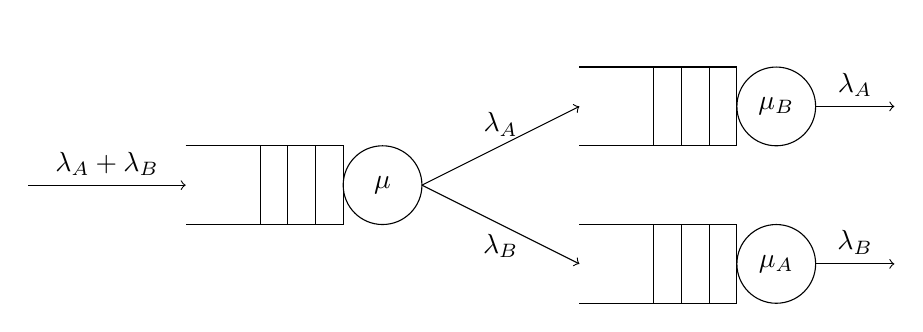
\begin{tikzpicture}[
->-/.style={decoration={markings, mark=at position .5 with {\arrow{stealth}}},
postaction={decorate}},
queuei/.pic={
  \draw%[line width=1pt]
    (0,-0.5) -- ++(2cm,0) -- ++(0,-1cm) -- ++(-2cm,0);
   \foreach \Val in {1,...,3}
     \draw ([xshift=-\Val*10pt]2cm,-0.5) -- ++(0,-1cm);
\draw (2.5,-1) circle [radius=0.5cm] node {#1};}
]
\path 
  (0,0) pic {queuei=$\mu$}
  (5,-1) pic {queuei=$\mu_A$}
  (5,1) pic {queuei=$\mu_B$};

\draw[->] (-2,-1)--(0,-1) node[midway, anchor=south] {$\lambda_A+\lambda_B$};
\draw[->] (3,-1)--(5,0) node[midway,above] {$\lambda_A$}; 
\draw[->] (3,-1)--(5,-2) node[midway,below] {$\lambda_B$}; 
\draw[->] (8,0)--(9,0) node[midway,above] {$\lambda_A$}; 
\draw[->] (8,-2)--(9,-2) node[midway,above] {$\lambda_B$}; 
%\draw[->-] (2.5,-0.5)-- ++(0,-1) -- ++(5.,0) -- ++(0, 1.5); 

\end{tikzpicture}
\caption{A queueing model of a paint factory.}
\label{fig:paint}
\end{figure}

To analyze how to control the average cycle time of an arbitrary job,
whether it is an A or a B job, we can use at least three models.
\begin{enumerate}
\item Model 1. Model all stations as $M/M/1$ queues. As, by
  assumption, the mixing station is an $M/M/1$ queue, its departure
  process is exponential with rate $\lambda_A + \lambda_B$, and of
  these departures, the type A jobs go to filling station A. Thus, we
  can compute the waiting times at stations $A$ and $B$ also. Finally,
  the average waiting time is given by the weighted average of the
  waiting times of the A and B jobs. One weak point of this model is
  the assumption of the exponentiality of the processing times at all
  stations. The data obtained at the paint factory tells that
  processing times are not really exponential.  However, we can model
  the processing times as expoential, and use the ideas of Section
  2.2. of Zijm's book to compute the waiting times.
\item Model 2. Model the second processing step as \emph{one} filling
  station, i.e., put an imaginary box around both filling stations A
  and B, and model it as one station with \emph{one} machine, but such
  that the capacity of this one machine is equal to the capacity of
  the two original filling machines. This is a simple model, but it
  approximates the two filling machines by one machine, and we know
  that multi-server queueing systems behave a bit different from
  single-server queueing systems. Besides that, there are two queues
  in front of the machines, but in this model we merge both queues
  into one.
\item Model 3. Model the second processing step as \emph{one} filling
  station, i.e., put an imaginary box around both filling stations A
  and B, but now model it as one station with \emph{two identical}
  machines.  This is also a simple model, but for this to work we need
  to assume that both machines have the same capacity, i.e.,
  processing speed. This assumption, however, is not satisfied in the
  paint factory.
\end{enumerate}

We see that all three models capture part of the real production
system, but they are also partly wrong.  To analyze the case it is
perhaps best to implement all three models and investigate to what
extent these models give similar or dissimilar results. Once we know
which models appears to give the most realistic, or robust, results,
we can use the models to obtain insight into the situation and provide
ideas how and where to improve the situation. Mind that in general it
is quite pointless to make very detailed models: often only gross data
is available, the data needed to estimate the parameters of
fine-grained models is simply not available, or need to be guesses.
As a conclusion, the analysis of a real situation often requires several
models, each with their own strengths and weaknesses.


\begin{exercise}
  It is mentioned in the text that there are $5M+M^2$ input parameters
  required to characterize an $M$ station network of $G/G/1$ queues. What are these parameters?
  \begin{hint}
 Check the formulas in the synthesis carefully.
  \end{hint}
  \begin{solution}
    \begin{enumerate}
    \item The routing matrix $P$ is $M$ times $M$, hence contains
      $M^2$ parameters, but often most of them will be zero.
    \item $\lambda_{0i}$ is the arrival rate of external jobs to station $i$, hence $M$ parameters.
    \item $C_{0i}^2$ is the SCV of the interarrival times at station
      $i$, hence $M$ parameters.
    \item $C_{si}^2$ is the SCV of the service times at station $i$,
      hence $M$ parameters.
    \item The expected service times $\E S_i$ at station $i$, 
      hence $M$ parameters.
    \item The number of servers $c_i$ at station $i$, hence $M$
      parameters.
    \end{enumerate}
  \end{solution}
\end{exercise}


%\begin{exercise}[use=false]
Here is an example to show how to use the formulas for the general open network.

\begin{exercise}
Consider a single-machine station with deterministic (very regular)
production times such that each job takes $S=10$ minutes. Jobs arrive
as a Poisson process with rate $\lambda=4$ per hour. Thus, we model
the station as an $M/D/1$ queue. Jobs fail with probability $1/5$ and
are sent back the machine for repair. The production times for repair
jobs are also 10 minutes.  What is the influence of faulty jobs on the
queueing times? 
\begin{hint}
Apply the formulas (2.30)--(2.33) of Zijm to a single station
  queueing network with rework.
\end{hint}
\begin{solution}
  First consider the situation without loss. Then
  \begin{equation*}
    \E{W_Q} = \frac{1+C_s^2}2 \frac{\rho}{1-\rho} \E S = \frac 12 \frac{2/3}{1/3} 10 = 10 \text{ min},
  \end{equation*}
since 
\begin{equation*}
\rho=\lambda \E S = 4 \frac{10}{60} = \frac 23,
\end{equation*}
This was easy. Now the case with rework.

Lets work from top to bottom of Section 2.4.2 of Zijm and compute
anything we need along the way. First, the departure SCV. Noting that
$i=1$ and $M=1$,
\begin{equation*}
  C_{d1}^2 
= (1-\rho_1^2)C_{a1}^2 + \rho_1^2 C_{s1}^2.
\end{equation*}
So, I need $\rho_1$. For this in turn I need $\lambda_1$. Now, from the traffic equations:
\begin{equation*}
  \lambda_ 1= \gamma + \frac15\lambda_1, 
\end{equation*}
hence, since $\gamma=4$,
\begin{equation*}
\lambda_1 = \frac 5 4 \gamma=5, \implies \rho_1 = \lambda_1 \E S=5\frac{10}{60}=\frac 56.
\end{equation*}
Thus, 
\begin{equation*}
  \begin{split}
  C_{d1}^2  
&= (1-\rho_1^2)C_{a1}^2 + \rho_1^2 C_{s1}^2\\
&= (1-\frac{25}{36})C_{a1}^2 + \frac{25}{36}\max\{0.2, 0\}\\
&= \frac{11}{36}C_{a1}^2 + \frac{5}{36}.
  \end{split}
\end{equation*}
Observe that we don't know $C_{a1}^2$ yet as it is a mix of the
external arrivals and the jobs that require rework. Also, we are, by
the explanation in Zijm's book, not allowed to take $C_{1s}^2=0$; we
need to use the suggested approximation to take
$C_s^2 = \max\{0.2, C_s^2\}$ in the formula, rather than $C_s^2$.

Next, splitting. We have
\begin{equation*}
  \begin{split}
  C_{11}^2 
&= P_{11}C_{d1}^2 + 1 - P_{11} = \frac{1}{5}C_{d1}^2 + \frac 45 \\
&=\frac{1}{5}\left(\frac{11}{36}C_{a1}^2 + \frac{5}{36}\right) + \frac 45 \\    
&\approx\frac{11/5}{36} C_{a1}^2 + \frac{1}{36} + \frac 45 \\
&\approx\frac{1}{18} C_{a1}^2 + \frac 45 \\
  \end{split}
\end{equation*}
since $11/5 \approx 2$ and $1/36 < 3\%$. 

Now merging.
\begin{equation*}
  C_{1a}^2 = w_1 \sum{i=0,1} Q_{i1} C_{i1}^2 + 1 - w_1.
\end{equation*}
Now, 
\begin{equation*}
  w_1^{-1} = 1 + 4(1-\rho_1)^2 (v_1-1),
\end{equation*}
and
\begin{equation*}
  v_1^{-1}=\sum_{i=0,1} Q_{i1}^2,
\end{equation*}
and 
\begin{equation*}
  Q_{i1} = \frac{\lambda_{i1}}{\lambda_1}.
\end{equation*}
Since $i=0$, for the external arrivals, or $i=1$ for the rework,
\begin{equation*}
  Q_{01} = \frac{\gamma}{\lambda_1} = \frac 45, \quad Q_{11}=\frac{\lambda_{11}}{\lambda_1} = \frac{1/5 \lambda_1 }{\lambda_1} = \frac 15.
\end{equation*}
Therefore
\begin{equation*}
  v_1^{-1}= \frac{16}{25}+\frac1{25} = \frac{17}{25},
\end{equation*}
and, since $\rho_1 = 5/6$,
\begin{equation*}
  \begin{split}
  w_1^{-1} 
&= 1 + 4(1-\rho_1)^2 (v_1-1) = 1 + 4\frac1{36}\left(\frac{25}{17}-1\right) \\
&= 1 + \frac1{9}\frac{8}{17} \approx 1 + \frac1{17} =\frac{18}{17}.
  \end{split}
\end{equation*}
Hence,
\begin{align*}
  C_{1a}^2 
&= w_1 \sum_{i=0,1} Q_{i1} C_{i1}^2 + 1 - w_1 \\
&= \frac{17}{18} \left(\frac 45 C_{01}^2 + \frac 1 5 C_{11}^2 \right) + 1 - \frac{17}{18}\\
&= \frac{17}{18} \left(\frac 45 1 + \frac 1 5 \left(\frac{1}{18} C_{a1}^2 + \frac 45\right)\right) + 1 - \frac{17}{18}\\
&\approx \frac 45 + \frac 1 5 \left(\frac{1}{18} C_{a1}^2 + \frac 45\right) \\
&\approx \frac 45 + \frac{1}{5\times 18} C_{a1}^2 + \frac 15 \\
&\approx 1 + \frac{1}{5\times 18} C_{a1}^2 \\
&\approx 1.
\end{align*}

So, provided all the estimations and approximations I used above are
not too way off, we see that we can take $C_{1a}^2=1$. And then, including the rework,
  \begin{equation*}
    \E{W_Q} = \frac{1+C_s^2}2 \frac{\rho}{1-\rho} \E S = \frac 12 \frac{5/6}{1/6} 10 = \frac 52 10 25 \text{ min}.
  \end{equation*}
  Thus, the average waiting time increases by a factor $2.5$ just
  because of the extra load of the rework.  

  Perhaps I should implement the above in python to deal with the
  numerical details.

  In the synthesis section in Section Zijm.2.4.2, all of the above
  algebra has been reduced to a set of linear equations to compute
  $C_{a,i}^2$ for stations $i=1,\ldots,M$.
\end{solution}
\end{exercise}


\begin{comment}
\begin{exercise}[use=false]
  \begin{enumerate}
  \item Three M/M/1 FIFO stations in tandem
  \item $\gamma_1 = 2/h$,  $\gamma_2 = 3/h$, $\gamma_3 = 1/h$
  \item All jobs from station 1 go to station 2
  \item jobs that arrive at 2 externally and those from station 1 move
    on to station 3
  \item 1 out of 4 jobs that complete service at station 3 need rework
    at station 2. The other  jobs leave the network
  \item The jobs that arrive at station 2 from station 3 leave the
    network after service at station 2.
  \item Determine the total arrival rates, i.e., $\lambda$, at each
    station. 
  \item Determine the routing matrix $P$. 
  % \item Suppose that at station 2, the average service time jobs from
  %   station~1 require 1 hour of service, the jobs that arrive directly
  %   at station 2 require 15 minutes of service, and the `rework' jobs
  %   require 5 minutes of work.
  \item Assume that $\E S_1 = 5$ min, $\E S_2 = 8$ min, and $\E S_3 =
    5$ min. Determine the expected number of jobs in the system. 
  \item Determine the density of the throughput time in the network
    of the jobs that arrive at station 1. Realize that part of these
    jobs have to undergo rework at station 2.
  \end{enumerate}
\begin{solution}
\TBD.
  \begin{enumerate}
  \item 
  The arrival rate at station 1 is $2$ per hour. Hence, $\rho_1 =
  \lambda_1/\mu_1 = \lambda_1 \E S_1 = 2/60 * 5 = 10/60 =
  1/10$. Hence, $L_{s,1} = \rho_1/(1-\rho_1)$.

  At station 3, only the jobs arrive from station 2 that did not come
  from station 3, plus $\gamma_3$. Hence, $\lambda_3 = \gamma_1 +
  \gamma_2 + \gamma_3 = 6$ per hour. Service time is $\E S_3 = 5$
  min. Hence, $\rho_3 = 6/60 * 5 = 30/60 = 1/2$. Then, $L_{s,2}$
  follows straightaway.

  Now station 2. This receives all jobs from station 1,
  i.e.,$\gamma_1$, plus $\gamma_2$, plus 25\% of the jobs that move on
  to station 3. Hence, $\lambda_2 = \gamma_1 + \gamma_2 + 1/4
  \lambda_3 = \gamma_1 + \gamma_2 + 1/4(\gamma_1 + \gamma_2 +
  \gamma_3) = 2 + 3 + (1+2+3)/4 = 5+6/4 = 5 + 3/2 = 6 1/2 = 13/2$ per
  hour. Therefore, $\rho_2 = \lambda_2 \E S_2 = 13/2/60 * 8 = 13*8/120
  = 104/120 = 52/60 = 26/30 = 13/15$.
\item   Simulate the network, and use the empirical distribution function to
  estimate the distribution function of the throughput times.
  \end{enumerate}
\end{solution}
\end{exercise}
\end{comment}



\Closesolutionfile{hint}
\Closesolutionfile{ans}

\opt{solutionfiles}{
\subsection*{Hints}
\input{hint}
\subsection*{Solutions}
\input{ans}
}
\clearpage
